\documentclass{article}
\usepackage[utf8]{inputenc}
\usepackage{amsthm, amsmath, amssymb, mathrsfs}
\usepackage{tikz}
\usepackage{graphics}
\usepackage{float}

\newtheorem{recap}{Recapitulation}

\title{Master 2 CSMI : EDP2\\Rapport TP2\\Résolution numérique de Saint-Venant}
\author{Romain Vallet}

\begin{document}

\maketitle

\subsubsection*{1.}

Voici le graphique du solveur de Riemann :

\begin{figure}[H]
    \centering
    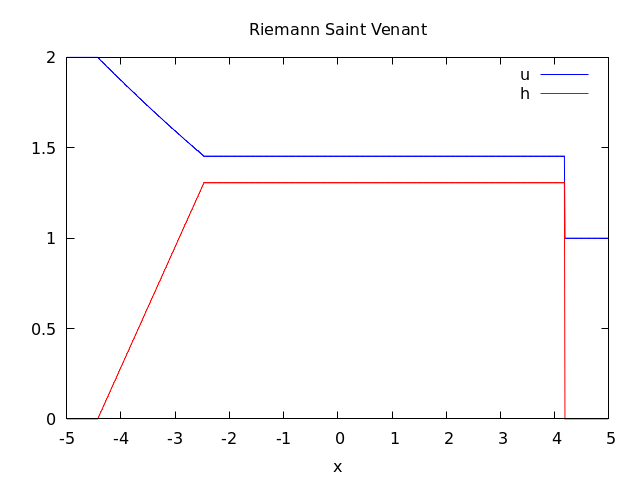
\includegraphics[scale=0.5]{figure/riemann.png}
    \caption{Solveur de Riemann}
\end{figure}

\subsubsection*{2.}

\subsubsection*{3.}

Nous pouvons poser comme conditions au bords :
\[ \left\{ \begin{matrix} 
    u_0^n = - u_1^n \\
    h_0^n = h_1^n \\
    u_N^n = - u_{N-1}^n \\
    h_N^n = h_{N-1}^n
\end{matrix} \right. \]

\subsubsection*{4.}

\subsubsection*{5.}

Nous posons $A(w) = f'(w) = \begin{pmatrix} 0 & 1 \\ -u^2+gh & 2u \end{pmatrix}$

Avec les valeurs propres de $A(w)$ : $\lambda_1(w) = u - \sqrt{gh}$ et $\lambda_2(w) = u + \sqrt{gh}$.

Nous posons la vitesse $\lambda = max(\rho(A(w_L), \rho(A(w_R)))) = max(|u_L|+\sqrt{gh_L}, \, |u_R|+\sqrt{gh_R})$

Le flux de Rusanov devient :
\begin{eqnarray*}
    f(w_L, w_R) &=& \frac{f(w_L) + f(w_R)}{2} - \frac{\lambda}{2} (w_R - w_L) \\
    &=& \begin{pmatrix} \frac{h_L u_L + h_R u_R}{2} - \frac{\lambda}{2} (h_R-h_L) \\
                        \frac{h_L u_L^2 + \frac{g h_L^2}{2} + h_R u_R^2 + \frac{g h_R^2}{2}}{2} - \frac{\lambda}{2} (h_R u_R - h_L u_L) \end{pmatrix}
\end{eqnarray*}

\subsubsection*{6.}

Nous remplaçons le solveur de Riemann exact par un solveur de Riemann approché.

Nous avons l'équation :
\[ \partial_t y \, + \, B(y) \partial_x y = 0 \text{ avec } y = \begin{pmatrix} h \\ u \end{pmatrix} \, , \, B(y)=\begin{pmatrix} u & h \\ g & u \end{pmatrix} \]

Nous remplaçons l'équation du solveur de Riemann avec $\bar{y} = \frac{y_L+y_R}{2}$ :
\[ \left\{ \begin{matrix} \partial_t y + B(y) \partial_x y = 0 \\ y(x,0) = \left\{ \begin{matrix} y_L \text{ si } x<0 \\ y_R \text{ si } x>0 \end{matrix} \right. \end{matrix} \right.
    \longrightarrow
    \left\{ \begin{matrix} \partial_t y + B(\bar{y}) \partial_x y = 0 \\ y(x,0) = \left\{ \begin{matrix} y_L \text{ si } x<0 \\ y_R \text{ si } x>0 \end{matrix} \right. \end{matrix} \right.
\]

Pour résoudre cette nouvelle équation, nous supposons que $B=B(\bar{y})$ est diagonalisable $B = P^{-1} D P$ avec $D = \begin{pmatrix} \lambda_1 & 0 \\ 0 & \lambda_2 \end{pmatrix}$.
Donc, nous avons :

\begin{eqnarray*}
    \partial_t y + P^{-1} D P \partial_x y = 0 \\
    \partial_t (Py) + D \partial_x (Py) = 0 \\
\end{eqnarray*}

Résoudre le problème de Riemann simplifié revient à résoudre avec le changement de variable $z = Py = \begin{pmatrix} z_1 \\ z_2 \end{pmatrix}$ :
\begin{eqnarray*}
\partial_t z + D \partial_x z = 0 \\
\Longrightarrow \left\{ \begin{matrix} \partial_t z_1 + \lambda_1 \partial_x z_1 = 0 \\
                        \partial_t z_2 + \lambda_2 \partial_x z_2 = 0
        \end{matrix} \right.
\end{eqnarray*}

Résoudre le problème de Riemann simplifié revient à résoudre deux problèmes de Riemann pour l'équation de transport en 1 dimension.

Le solveur de Riemann pour une équation de transport en 1 dimension s'écrit :
\[ R(u_L, u_R, 0) = \frac{u_L+u_R}{2} - \frac{sgn(c)}{2} (u_R-u_L) \]

Nous pouvons reporter ce résultat pour l'équation de Saint-Venant, le solveur simplifié s'écrit : 
\[ \tilde{R}(y_L, y_R, 0) = \frac{y_L+y_R}{2} - \frac{sgn(B)}{2} (y_R-y_L) \]

Avec $sgn$ tel que $sgn(B) = sign(P^{-1} \begin{pmatrix} \lambda_1 & 0 \\ 0 & \lambda_2 \end{pmatrix} P) = P^{-1} \begin{pmatrix} sgn(\lambda_1) & 0 \\ 0 & sgn(\lambda_2) \end{pmatrix} P$
\newline

Pour le cas de l'équation de Saint-Venant :
\[ B(\bar{y}) = \begin{pmatrix} \bar{u} & \bar{h} \\ g & \bar{u} \end{pmatrix} = P^{-1} \begin{pmatrix} \lambda_1 & 0 \\ 0 & \lambda_2 \end{pmatrix} P \]

Avec :
\begin{itemize}
    \item $\lambda_1 = \bar{u} - \sqrt{g \bar{h}}$
    \item $\lambda_2 = \bar{u} + \sqrt{g \bar{h}}$
    \item $P = \begin{pmatrix} r_1 & r_2 \end{pmatrix} = \begin{pmatrix} -\sqrt{\bar{h}} & \sqrt{\bar{h}} \\ \sqrt{g} & \sqrt{g} \end{pmatrix}$
\end{itemize}

Alors :
\[ sgn(B(\bar{y})) = \left\{ \begin{matrix}
        I \text{ si } \lambda_1, \lambda_2 > 0 \\
        -I \text{ si } \lambda_1, \lambda_2 < 0 \\
        \begin{pmatrix} 0 & 1 \\ 1 & 0 \end{pmatrix} \text{ si } \lambda_1 < 0, \lambda_2 > 0
\end{matrix} \right. \]

\underline{Remarque :} $\lambda_1 > 0$ et $\lambda_2 < 0$ est impossible.
\newline

Le solveur de Riemann devient :
\[ \tilde{R}(y_L, y_R, 0) \left\{ \begin{matrix} 
        y_L \text{ si } \lambda_1, \lambda_2 > 0 \\
        y_R \text{ si } \lambda_1, \lambda_2 < 0 \\
        y^* \text{ si } \lambda_1 < 0, \lambda_2 > 0
\end{matrix} \right. \]

Avec  $y^* = \begin{pmatrix} \frac{h_L+h_R}{2} - \frac{\bar{h}}{2 \sqrt{g \bar{h}}} (u_R-u_L) \\ \frac{u_R+u_L}{2} - \frac{g}{2 \sqrt{g \bar{h}}} (h_R-h_L) \end{pmatrix}$
\newline

\underline{Conclusion :} le flux de la méthode VFRoe est $f(y_L, y_R) = \tilde{R}(y_L, y_R, 0)$.


\end{document}
